\chapter{Introduction}

\gls{ml} has become a powerfull tool for solving a wide variety of problems. One such field that has been particulary challenging is \gls{co}. 

\section{Background}

This chapter is dedicated to all the knowledge and background research that was required for this project.

\subsection{Listings}
You can do listings, like in Listing~\ref{ListingReference}
\begin{lstlisting}[caption={[Short caption]Look at this cool listing. Find the rest in Appendix~\ref{Listing}},label=ListingReference]
$ java -jar myAwesomeCode.jar
\end{lstlisting}

You can also do language highlighting for instance with Golang:
And in line~\ref{LineThatDoesSomething} of Listing~\ref{ListingGolang} you can see that we can ref to lines in listings.

\begin{lstlisting}[caption={Hello world in Golang},label=ListingGolang,escapechar=|]
package main

import "fmt"

func main() {
    fmt.Println("hello world") |\label{LineThatDoesSomething}|
}

\end{lstlisting}

\subsection{Figures}

Example of a centred figure
\begin{figure}[H]
    \centering
    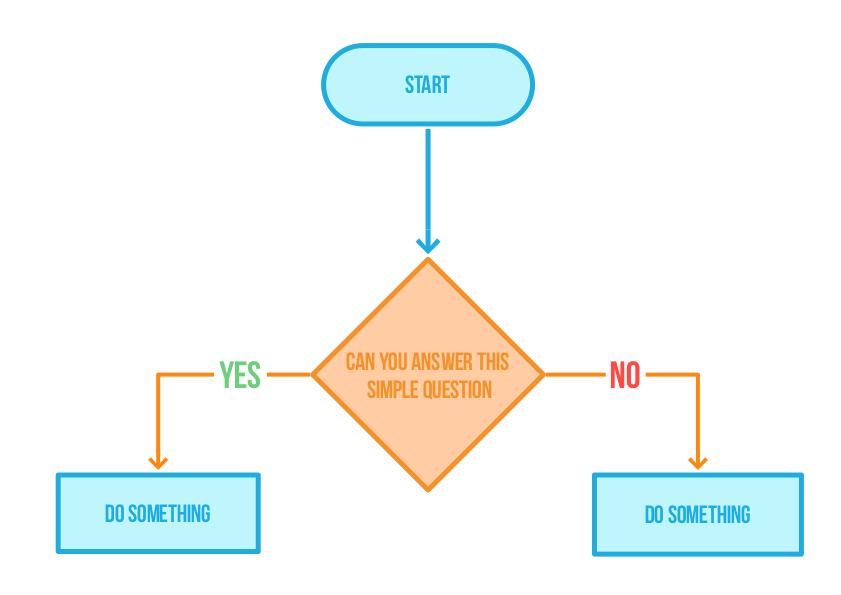
\includegraphics[scale=0.5]{figures/Flowchart}
    \caption{Caption for flowchart}
  	\medskip 
	\hspace*{15pt}\hbox{\scriptsize Credit: Acme company makes everything \url{https://acme.com/}}
    \label{FlowchartFigure}
\end{figure}

\subsection{Tables}

We can also do tables. Protip: use \url{https://www.tablesgenerator.com/} for generating tables.
\begin{table}[H]
\centering
\caption{Caption of table}
\label{TableLabel}
\begin{tabular}{|l|l|l|}
\hline
Title1 & Title2 & Title3 \\ \hline
data1  & data2  & data3  \\ \hline
\end{tabular}
\end{table}

\subsection{\gls{git}}

\gls{git} is fun, use it!